\documentclass[UTF8,aspectratio=169,11pt]{ctexbeamer}

% ========== Theme ==========
\usetheme{Madrid}
\usecolortheme{whale}
\setbeamertemplate{navigation symbols}{}
\setbeamertemplate{footline}[frame number]

% ========== Packages ==========
\usepackage{tikz}
\usetikzlibrary{arrows.meta, positioning, shapes.geometric, calc, fit, backgrounds}
\usepackage{booktabs}
\usepackage{graphicx}
\usepackage{amsmath}
\usepackage{xcolor}
\usepackage{array}

% ========== Colours ==========
\definecolor{highlight}{RGB}{220, 70, 70}
\definecolor{completed}{RGB}{80, 185, 100}
\definecolor{pending}{RGB}{180, 180, 180}
\definecolor{inprogress}{RGB}{90, 140, 240}

% ========== Title ==========
\title{面向灵巧操作的闭环控制项目汇报}
\subtitle{基于深度学习的 BCI 机械臂闭环控制系统}
\author{}
\institute{RL / Embodied AI / Robust Control}
\date{2026年5月}

\begin{document}

\begin{frame}
    \titlepage
    \vspace{-4mm}
    \begin{center}
        \small
        \parbox{0.92\textwidth}{\centering
        \textbf{一句话总结：}我采用迁移学习与强化学习方法，使用 \textbf{EEGTransformer} 识别 EEG 运动想象意图，并在 PyBullet / OpenBCI 控制链路中，通过 \textbf{Transformer DQN} 闭环策略网络控制机械臂末端完成目标到达。}
    \end{center}
\end{frame}

\begin{frame}[shrink=8]{1. 我解决的核心问题}

    \begin{block}{我解决的问题}
        我解决的是\textbf{噪声感知下的闭环决策控制}：当 EEG 分类并不完美时，控制策略仍能利用状态反馈持续纠错，并稳定完成目标到达。
    \end{block}

    \vspace{2mm}
    \begin{exampleblock}{项目支撑}
        \begin{itemize}
            \item \textbf{方法侧}：EEGTransformer + 迁移学习负责意图感知，Transformer DQN 负责闭环控制
            \item \textbf{结果侧}：在 82.22\% 分类精度下，闭环控制仍达到约 99\% 目标到达率
            \item \textbf{工程侧}：完成训练、消融、仿真评估、OpenBCI 与机械臂接口
        \end{itemize}
    \end{exampleblock}

    \vspace{2mm}
    \begin{alertblock}{能力迁移}
        这个能力可以迁移到灵巧操作中的 observation design、reward engineering、policy optimization、Sim2Real 和多模态鲁棒控制。
    \end{alertblock}
\end{frame}

\begin{frame}[shrink=8]{2. 能力对应与项目支撑}
    \begin{table}
        \centering
        \scriptsize
        \renewcommand{\arraystretch}{1.18}
        \begin{tabular}{p{3.0cm}p{7.7cm}}
            \toprule
            \textbf{核心能力} & \textbf{项目支撑} \\
            \midrule
            强化学习训练能力 &
            将控制任务建模为 MDP；设计 observation、action、reward；比较 CNN+LSTM、Light Transformer、Transformer DQN；完成端到端评估。 \\
            \addlinespace
            训练稳定性与 Debug &
            针对分类噪声、轨迹震荡、越界、稀疏到达奖励设计 reward shaping 和闭环纠错机制。 \\
            \addlinespace
            Foundation Policy 融合理解 &
            当前系统已是“感知模块 + 低层策略”的组合；可自然迁移到 VLA 负责高层任务理解、RL 负责低层接触控制。 \\
            \addlinespace
            多模态感知 &
            当前使用 EEG 预测、置信度和机械臂状态；灵巧手场景可扩展到 vision、tactile、force、proprioception。 \\
            \addlinespace
            仿真到部署 &
            已完成 PyBullet 仿真训练和 OpenBCI / SO-101 接口；方法论可迁移到 MuJoCo、Isaac Gym、ManiSkill。 \\
            \addlinespace
            Research Engineer 能力 &
            不是只读论文，而是实现模型、跑实验、做消融、分析失败模式，并把软件链路接到硬件接口。 \\
            \bottomrule
        \end{tabular}
    \end{table}
\end{frame}

\begin{frame}{3. 系统整体架构}
    \begin{center}
        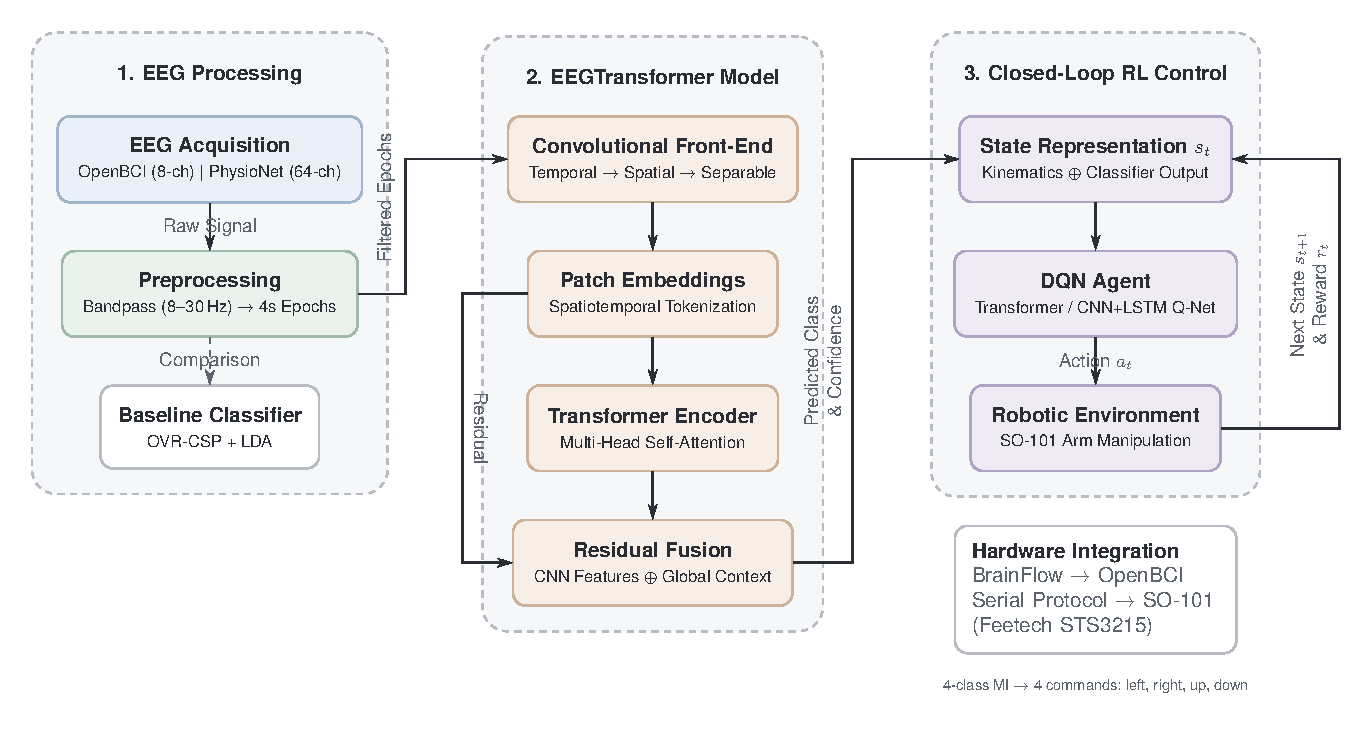
\includegraphics[width=0.94\textwidth,height=0.68\textheight,keepaspectratio]{architecture_diagram.pdf}
    \end{center}

    \vspace{1mm}
    \begin{center}
        \small
        系统抽象为：噪声感知表征 $\rightarrow$ 状态构建 $\rightarrow$ RL 低层策略 $\rightarrow$ 机器人执行与环境反馈。
    \end{center}
\end{frame}

\begin{frame}[shrink=8]{4. RL 能力：MDP、Reward、Action 与训练稳定性}

    \begin{columns}[T]
        \column{0.49\textwidth}
        \textbf{当前项目中的 MDP 设计}
        \begin{itemize}
            \item \textbf{Observation}：末端位置、目标位置、距离、EEG 预测类别、分类置信度
            \item \textbf{Action}：左 / 右 / 上 / 下离散动作，用于验证闭环纠错
            \item \textbf{Reward}：到达目标奖励、距离改善奖励、步数惩罚、震荡惩罚、越界惩罚
            \item \textbf{Policy}：CNN+LSTM、Light Transformer、Transformer DQN 对比
        \end{itemize}

        \column{0.49\textwidth}
        \textbf{迁移到灵巧操作的做法}
        \begin{itemize}
            \item 高维连续动作：优先考虑 PPO / SAC / TD3，而不是直接沿用 DQN
            \item 稀疏奖励：用 curriculum、dense shaping、success classifier 或 hindsight 风格采样缓解
            \item 接触不稳定：把 slip、force、contact consistency、joint limit 加入 observation / reward
            \item 训练稳定性：做 seed sweep、ablation、learning curve、failure case replay
        \end{itemize}
    \end{columns}

    \vspace{2mm}
    \begin{alertblock}{方法迁移}
        我用 DQN 完成了离散闭环控制验证；面对多指灵巧手的高自由度连续控制，我会把同样的 MDP / reward / debug 方法迁移到 PPO、SAC 或 TD3。
    \end{alertblock}
\end{frame}

\begin{frame}[shrink=8]{5. VLA / Foundation Policy + RL 的融合理解}

    \begin{center}
        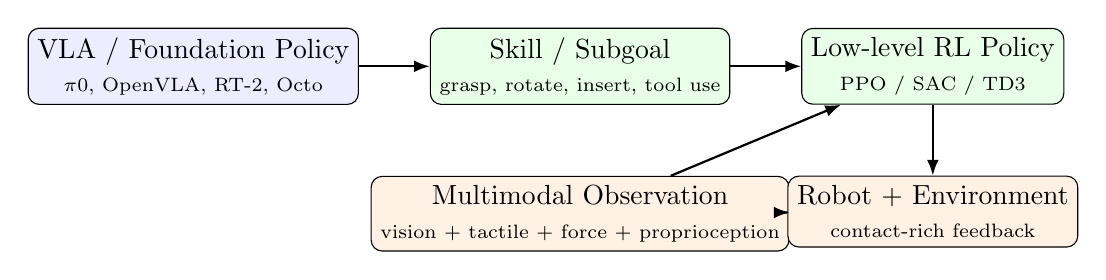
\begin{tikzpicture}[
            node distance=9mm,
            block/.style={draw, rounded corners, align=center, minimum width=2.7cm, minimum height=0.8cm, fill=blue!7},
            policy/.style={draw, rounded corners, align=center, minimum width=2.8cm, minimum height=0.8cm, fill=green!9},
            data/.style={draw, rounded corners, align=center, minimum width=2.7cm, minimum height=0.8cm, fill=orange!10},
            arrow/.style={-{Latex[length=2mm]}, thick}
        ]
            \node[block] (vla) {VLA / Foundation Policy\\{\scriptsize $\pi0$, OpenVLA, RT-2, Octo}};
            \node[policy, right=of vla] (skill) {Skill / Subgoal\\{\scriptsize grasp, rotate, insert, tool use}};
            \node[policy, right=of skill] (rl) {Low-level RL Policy\\{\scriptsize PPO / SAC / TD3}};
            \node[data, below=of skill] (obs) {Multimodal Observation\\{\scriptsize vision + tactile + force + proprioception}};
            \node[data, below=of rl] (robot) {Robot + Environment\\{\scriptsize contact-rich feedback}};
            \draw[arrow] (vla) -- (skill);
            \draw[arrow] (skill) -- (rl);
            \draw[arrow] (obs) -- (rl);
            \draw[arrow] (rl) -- (robot);
            \draw[arrow] (robot) -- (obs);
        \end{tikzpicture}
    \end{center}

    \vspace{1mm}
    \begin{columns}[T]
        \column{0.49\textwidth}
        \textbf{我的理解}
        \begin{itemize}
            \item VLA 适合做任务理解、语言条件化、视觉语义 grounding
            \item Diffusion Policy / ACT 适合从演示中学习短程动作分布
            \item RL 适合做接触恢复、稳定抓取、失败纠正和长期 reward 优化
        \end{itemize}

        \column{0.49\textwidth}
        \textbf{系统对应}
        \begin{itemize}
            \item EEG 分类器类似一个不完美的高层意图 / 感知信号
            \item DQN 不盲目执行分类结果，而是在闭环状态中持续纠错
            \item 这与“Foundation Policy 给先验，RL 做低层精修”是同一类系统思想
        \end{itemize}
    \end{columns}
\end{frame}

\begin{frame}[shrink=8]{6. 迁移到灵巧手 / Contact-rich Manipulation 的方案}

    \begin{columns}[T]
        \column{0.49\textwidth}
        \textbf{任务建模}
        \begin{itemize}
            \item \textbf{稳定抓取}：grasp success、slip penalty、force balance
            \item \textbf{手内旋转}：object pose progress、contact maintenance、joint limit penalty
            \item \textbf{工具使用}：long-horizon subgoal、skill chaining、failure recovery
            \item \textbf{高自由度控制}：关节目标、delta pose、impedance / residual action
        \end{itemize}

        \column{0.49\textwidth}
        \textbf{训练与部署}
        \begin{itemize}
            \item 仿真平台：MuJoCo / Isaac Gym / ManiSkill / RoboSuite
            \item 算法路线：IL 初始化 + RL fine-tuning，或 VLA 生成 subgoal + RL controller
            \item Sim2Real：domain randomization、系统辨识、触觉 / 力反馈校准
            \item Debug 重点：接触抖动、探索不足、reward hacking、策略过拟合
        \end{itemize}
    \end{columns}

    \vspace{2mm}
    \begin{exampleblock}{迁移路径}
        我会把已有的闭环控制、reward engineering、训练消融和部署接口经验，迁移到 Allegro / Shadow / Leap / Inspire 等灵巧手平台的多模态接触控制任务。
    \end{exampleblock}
\end{frame}

\begin{frame}[shrink=8]{7. 感知模块：EEGTransformer 与迁移学习}

    \begin{columns}[T]
        \column{0.5\textwidth}
        \textbf{分类器设计}
        \begin{itemize}
            \item \textbf{CNN 前端}：提取运动皮层相关空间模式
            \item \textbf{Transformer 编码器}：建模 4 秒 EEG 序列的长时依赖
            \item \textbf{迁移学习}：跨被试预训练，再做个体微调
            \item \textbf{部署考虑}：保留置信度输出，供控制策略判断感知可靠性
        \end{itemize}

        \vspace{2mm}
        \begin{exampleblock}{机器人场景类比}
            EEG 的跨用户差异，类似机器人中的跨环境、跨物体、跨传感器分布变化；迁移学习对应快速适配和低校准成本。
        \end{exampleblock}

        \column{0.48\textwidth}
        \textbf{关键结果}
        \begin{itemize}
            \item BCI IV-2a（22 通道，4 分类）：\textbf{73.80\%}
            \item BCI IV-2b（3 通道，2 分类）：\textbf{82.87\%}
            \item PhysioNet 跨被试训练：\textbf{56.54\%}
            \item PhysioNet 微调后：\textbf{88.78\%}
        \end{itemize}

        \vspace{2mm}
        \begin{alertblock}{核心结论}
            个体微调带来约 \textbf{32 个百分点}提升，说明预训练模型学到了可迁移表征，而不是只记住单个被试分布。
        \end{alertblock}
    \end{columns}
\end{frame}

\begin{frame}[shrink=8]{8. 关键量化结果：从感知到决策}
    \begin{columns}[T]
        \column{0.48\textwidth}
        \textbf{PhysioNet 分类结果}
        \begin{table}
            \centering
            \scriptsize
            \begin{tabular}{p{2.9cm}cc}
                \toprule
                训练方式 & 精度(\%) & 备注 \\
                \midrule
                跨被试训练 & 56.54 & 109人 pooled \\
                个体微调 & \textbf{88.78} & 10人, 5-fold CV \\
                \bottomrule
            \end{tabular}
        \end{table}

        \vspace{2mm}
        \begin{exampleblock}{含义}
            感知模型具备可迁移表征，经过少量个体校准后可以显著提升性能。
        \end{exampleblock}

        \column{0.48\textwidth}
        \textbf{DQN 架构对比}
        \begin{table}
            \centering
            \scriptsize
            \begin{tabular}{lccc}
                \toprule
                架构 & 时间(s) & 到达率 & Reward \\
                \midrule
                CNN+LSTM & 111.7 & 97\% & 8.79 \\
                Light Trans. & 134.0 & 99\% & 10.07 \\
                \textbf{Transformer DQN} & \textbf{177.8} & \textbf{100\%} & \textbf{10.39} \\
                \bottomrule
            \end{tabular}
        \end{table}

        \vspace{2mm}
        \begin{alertblock}{含义}
            时序建模不仅用于感知，也用于决策；Transformer DQN 在最终控制表现上最好。
        \end{alertblock}
    \end{columns}
\end{frame}

\begin{frame}[shrink=8]{9. 8 通道部署与 Observation 取舍}

    \begin{columns}[T]
        \column{0.48\textwidth}
        \textbf{通道压缩策略}
        \begin{itemize}
            \item 通过 leave-one-channel-out 消融评估各电极重要性
            \item 结果表明 \textbf{C3} 是最关键通道
            \item 构造 OpenBCI 兼容的 8 通道集合：
            \item \scriptsize{\texttt{C3, C4, FC3, FC4, CP3, CP4, Cz, FCz}}
        \end{itemize}

        \vspace{2mm}
        \textbf{预处理取舍}
        \begin{itemize}
            \item 8--30 Hz 带通滤波平均提升：\textbf{+18.44\%}
            \item ICA 额外增益只有：\textbf{+1.51\%}
            \item 最终主流程保留 \textbf{bandpass-only}
        \end{itemize}

        \column{0.48\textwidth}
        \begin{center}
            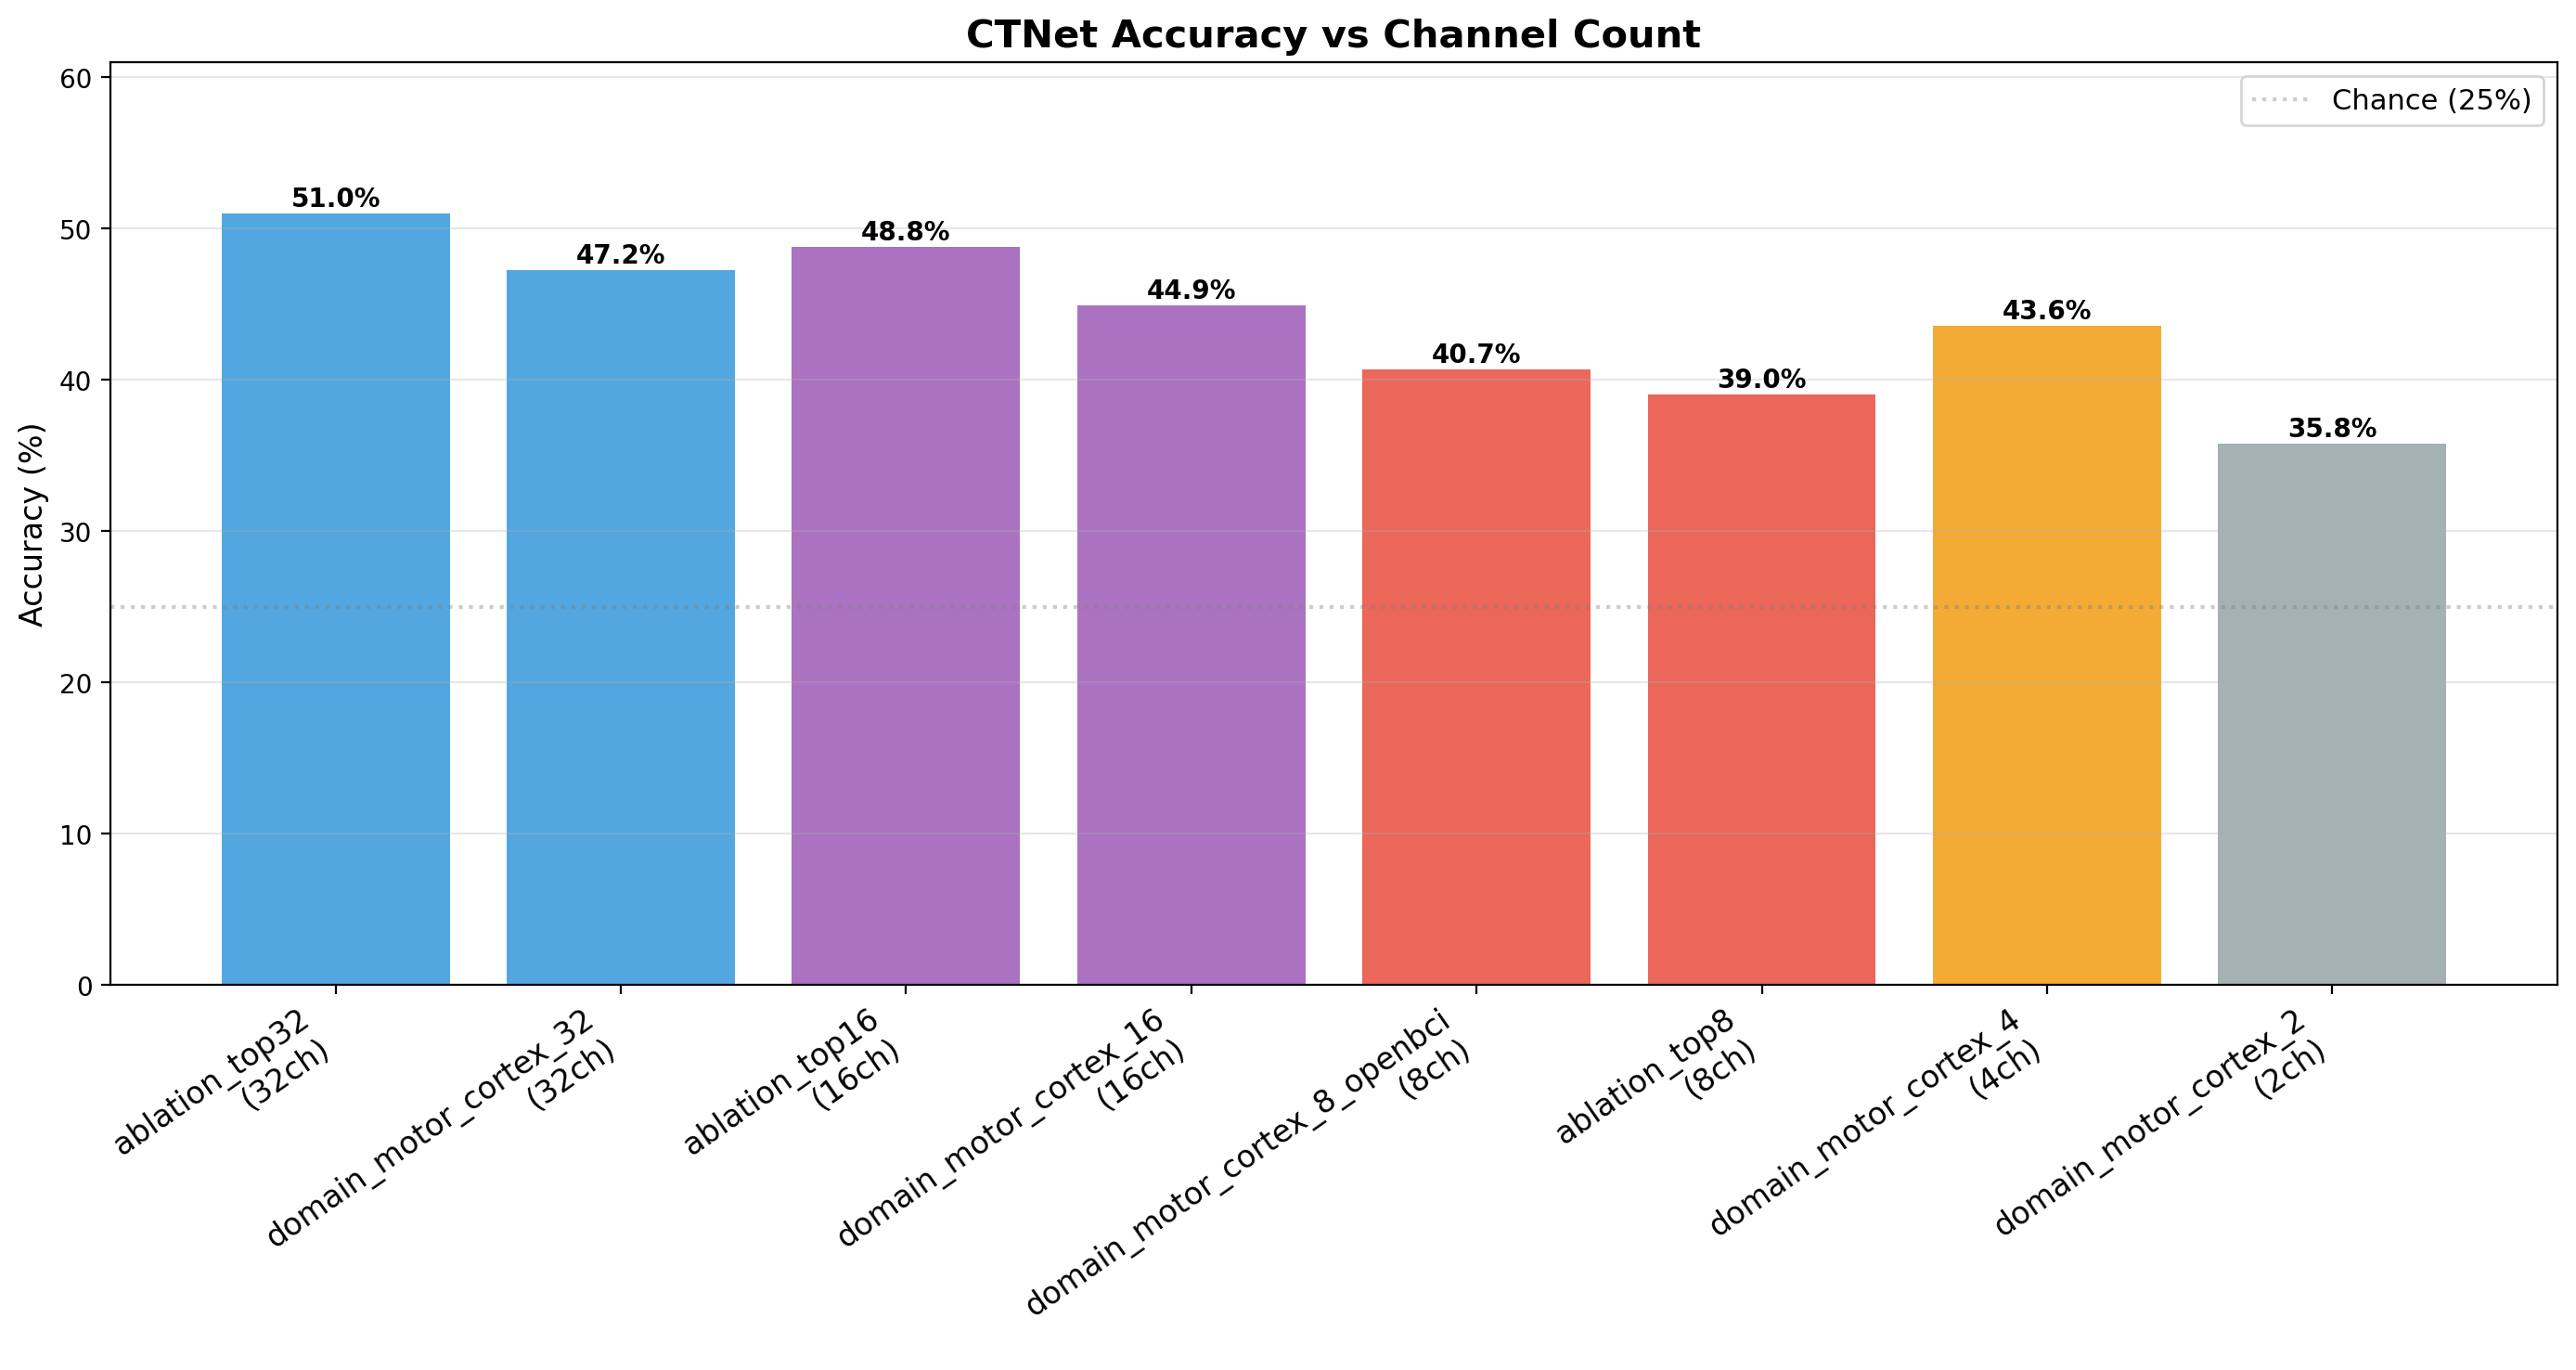
\includegraphics[width=\textwidth]{../03_Experiments/Channel_Reduction/channel_reduction/channel_reduction_comparison.png}
        \end{center}

        \vspace{1mm}
        \begin{alertblock}{Observation 设计启发}
            这对应机器人里的 observation space design：不是把所有传感器无差别堆进去，而是通过消融找到稳定、低成本、可部署的状态输入。
        \end{alertblock}
    \end{columns}
\end{frame}

\begin{frame}[shrink=8]{10. 端到端结果：感知有噪声，控制仍然稳定}

    \begin{columns}[T]
        \column{0.5\textwidth}
        \begin{center}
            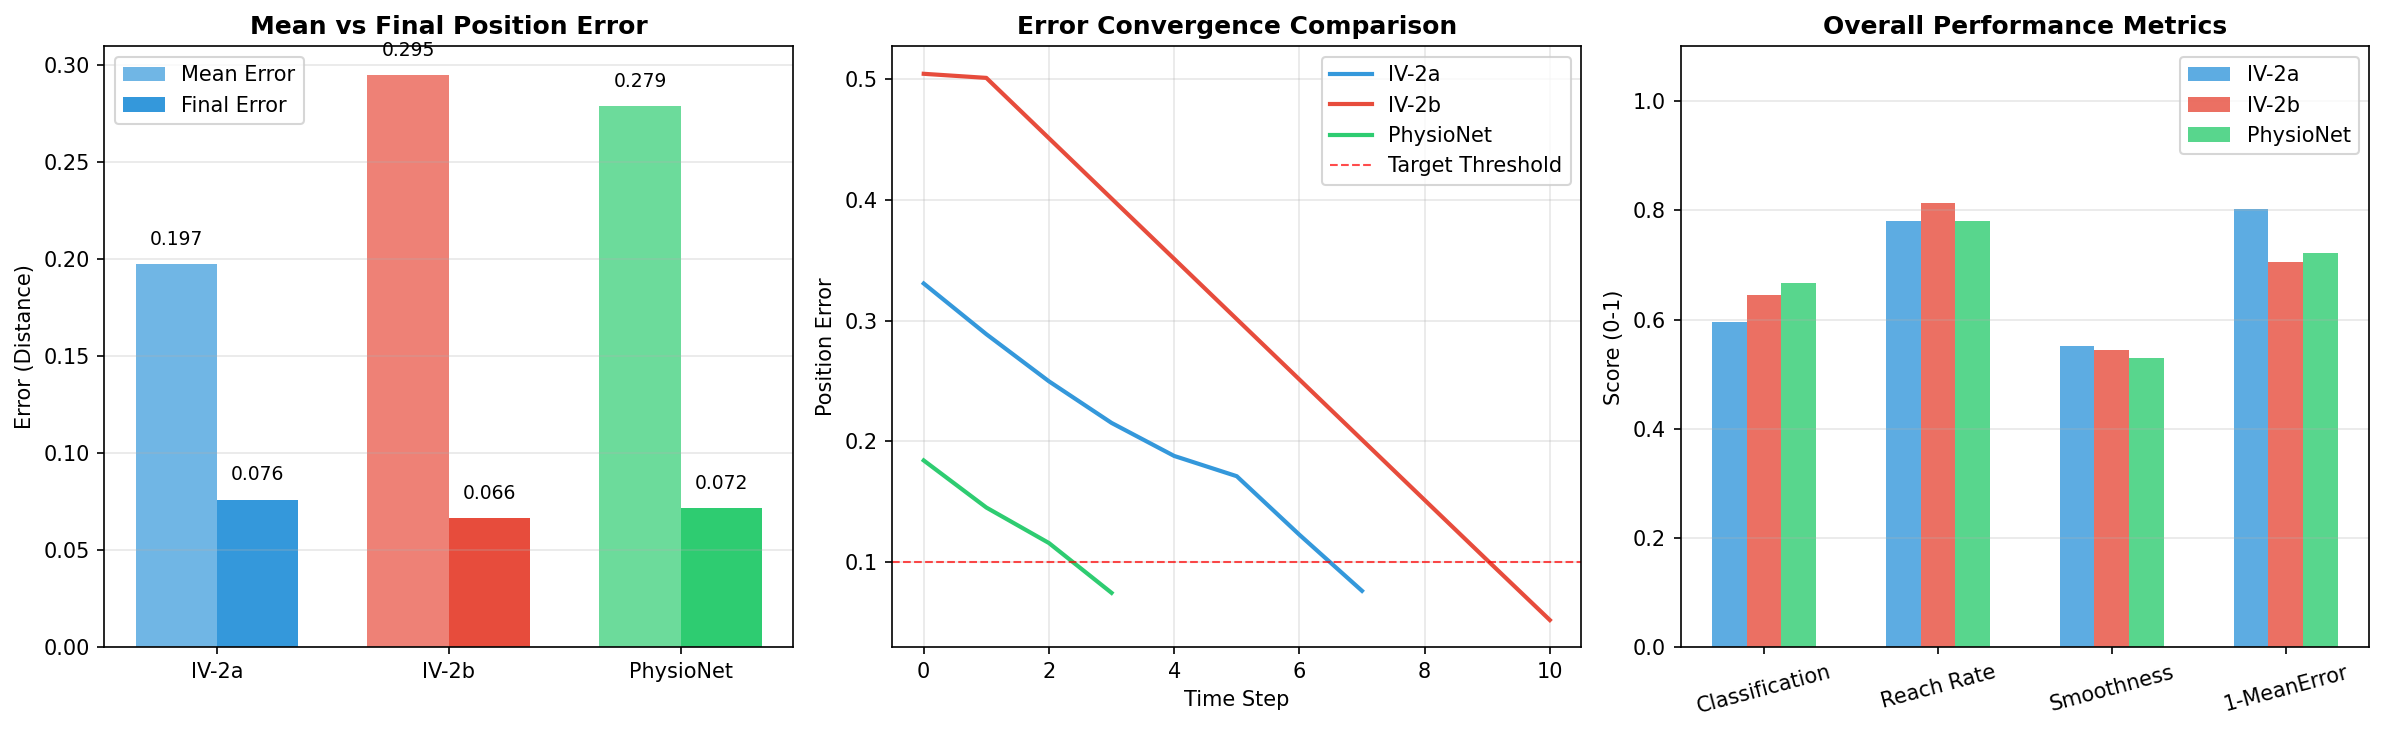
\includegraphics[width=\textwidth]{../03_Experiments/E2E_Evaluation/rl_control_test/overall_performance.png}
        \end{center}

        \column{0.48\textwidth}
        \textbf{报告中的原始结果表}
        \begin{table}
            \centering
            \scriptsize
            \begin{tabular}{lcccc}
                \toprule
                Agent State & 维度 & 到达率 & Reward & 时间(s) \\
                \midrule
                Arm only & 5 & 99.0\% & 8.71 & 1130 \\
                Arm + EEG & 7 & 98.7\% & 8.59 & \textbf{668} \\
                \bottomrule
            \end{tabular}
        \end{table}

        \vspace{1mm}
        \textbf{EEG 分类精度：} \textbf{82.22\%}

        \vspace{2mm}
        \begin{alertblock}{核心结论}
            闭环 RL 能够吸收分类误差，而不是机械执行分类结果。对灵巧操作来说，这对应“感知和接触都不完美时，策略仍要稳定完成任务”。
        \end{alertblock}
    \end{columns}
\end{frame}

\begin{frame}[shrink=7]{11. 工程实现范围与验证边界}

    \begin{columns}[T]
        \column{0.48\textwidth}
        \textbf{我实际完成的部分}
        \begin{itemize}
            \item MNE / PyTorch 的预处理、训练、微调和评估
            \item PyBullet 仿真环境与强化学习训练
            \item BrainFlow 接入 OpenBCI 实时 EEG 流
            \item SO-101 机械臂串口控制链路
            \item 通道压缩、预处理消融、端到端控制评估
        \end{itemize}

        \column{0.5\textwidth}
        \textbf{验证范围}
        \begin{itemize}
            \item 当前项目已完成软件链路与仿真验证
            \item 已实现 OpenBCI 与机械臂接口，但未做真人在线闭环实验
            \item 当前实物接口集中在 BCI 机械臂链路；灵巧手方向对应 RL 控制、系统工程和鲁棒决策能力迁移
        \end{itemize}

        \vspace{2mm}
        \begin{exampleblock}{总结}
            我能贡献的是：把论文方法真正复现、训练、调参、消融和接入系统；在灵巧操作场景下，我会把这套能力迁移到 VLA + RL、多模态感知和 contact-rich manipulation 的落地验证中。
        \end{exampleblock}
    \end{columns}
\end{frame}

\end{document}
